\chapter{Adatbázis}
\label{chap:fejezet3}

\section{Az adatbázis típusa}
Először is el kell döntenünk, hogy milyen adatbázist fogunk használni a fejleszteni kívánt alkalmazásunkhoz. Ennek sok szempontja lehet, például hogy mekkora mennyiségű adattal szeretnénk dolgozni, vagy hogy mennyire kell gyorsnak lennie a lekérdezéseknek.

\begin{figure}[H]
	\caption{Példa az adatbázis beállításra}
	\label{fig:adatbazisbeallitas}
	\centering
	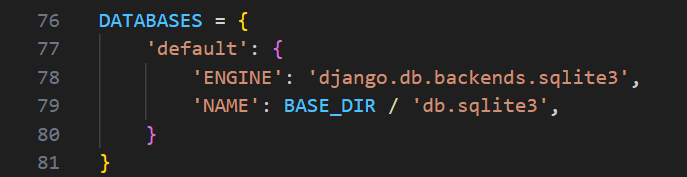
\includegraphics[width=1.0\textwidth]{database_setting.png}
\end{figure}

A szakdolgozatomban a Django beépített adatbázisát használtam, ami sqlite3, mivel egy fogászati rendelőnek nincsen nagyon nagy adatforgalma, így elegendő hozzá ez a fajta adatbázis. A 3.1 ábrán látható egy példa az adatbázis típusának beállítására. Ezt a beállítást a settings.py fájlban kell megadni, ami az én alkalmazásomban a projekt fő mappáján belüli "rendelo" nevú mappában található.

\section{Az adatbázis felépítése}
Az adatbázis típusának kiválasztása után a legfontosabb rész következik: Felépíteni az adatbázis szerkezetét. Mivel ORM technológiát használ a keretrendszerünk így szerencsére nincs szükségünk SQL ismeretekre ennek a műveletnek a végrehajtásához. Django-ban minden alkalmazásnak van egy (vagy több) models.py nevű fájlja. Ebbe importálnunk kell a Django models modulját, amit így tehetünk meg:\\
\texttt{from django.db import models}
\\
Ezután Python osztályként beleírhatjuk a fájlba a tárolni kívánt adatok tulajdonságait. Az ORM-ben az adatbázis táblák oszlopait a Python osztályaink adják meg, és az adatbázis rekordok ezeknek a példányaiból keletkeznek. Minden modell osztálynak közvetlenül, vagy közvetetten a \texttt{models.Model} modulból kell származnia.

\begin{figure}[H]
	\caption{Példa az adatbázis modell leírására}
	\label{fig:adatbazismodell}
	\centering
	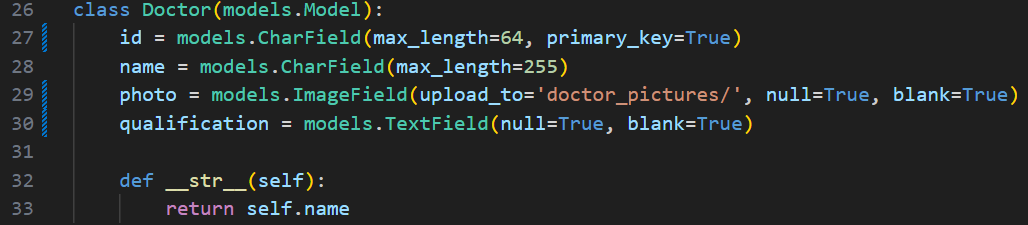
\includegraphics[width=1.0\textwidth]{database_model_example.png}
\end{figure}

A szakdolgozatomban egyértelmű volt, hogy FHIR szabványú adatbázissal kell dolgoznom, mivel az egészségügyi alkalmazásoknak ez a szabványa. Azért éri meg így kialakítani az adatbázist, mert ezzel a módszerrel az összes egészségügyi rendszerrel kompatibilis rendszert hozhatunk létre. A 3.2. ábrán látható az egyik FHIR szabványú modell osztály a szakdolgozatomból.\\
A modellek megírása nem volt egyszerű, mivel meg kellett oldanom a profilkezelést és az autentikációt az alkalmazásban, viszont szabványosnak kellett maradnia. Ezzel az a probléma, hogy az FHIR szabvány nem támogat profilkezelést.\\
Az alkalmazás modell osztályai:
\begin{itemize}
	\item RendeloUser
	\item Patient
	\item Doctor
	\item Treatment
	\item Appointment
	\item WorkingHours
	\item PaymentStatus
\end{itemize}

\subsection{Profilkezelés}

\begin{figure}[H]
	\caption{A felhasználói profilokat tároló modell}
	\label{fig:profilmodell}
	\centering
	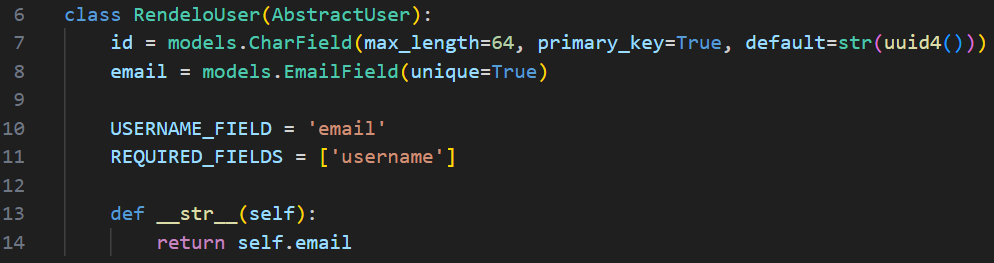
\includegraphics[width=1.0\textwidth]{abstractuser_model.png}
\end{figure}

Az alkalmazásomban három felhasználói jogosultságú profil elérhető:

\begin{itemize}
	\item Superuser: Adminisztrátor akinek mindenhez van joga, bármilyen adatot törölhet, meg van valósítva a számára egy külön "Admin" nevű oldal amin az adatok kezeléséhez hozzáfér, és beléphet a Django beépített adminisztrátori felületére is.
	\item Staff: A fogászati rendelő orvosainak a jogosultságával rendelkezik. Ezeket a profilokat az adminisztrátor tudja létrehozni az "Admin" oldalon. Minden ilyen profil megjelenik orvosként az orvosok kiválasztásánál az időpontfoglalás során. Joga van megtekinteni a páciensek kezeléstörténetét, és szerkeszteni azt. Joga van az összes hozzá foglalt időpont megtekintésére, a páciensek adatainak lekérdezésére, és a saját munkaidejének a beállítására.
	\item User: A páciensek felhasználói fiókjai, a Regisztrációs oldalon hozhatók létre. Az időpontfoglaláshoz csak ezeknek a fiókoknak van joga, emellett megtekinthetik a saját kezeléstörténetüket és az időpontjaikat, illetve le is mondhatják azokat.
\end{itemize}

A profilokat a 3.3. ábrán látható RendeloUser osztály tárolja. Az osztály az AbstractUser-ből származik, ami a Django beépített autentikációs rendszerébe tartozik. Amikor létrehozunk az alkalmazásban egy bármilyen jogosultsággal rendelkező profilt, akkor ez az osztály fogja tárolni a bejelentkezéshez szükséges adatainkat. Superuser esetén csak ez az egy objektum tartozik a profilunkhoz, mivel az adminisztrátor nem orvos, és nem páciens, nincs szüksége további adat tárolására.

Ha az adminisztrátor létrehoz egy új orvosnak egy profilt az alkalmazásban, akkor először is létrejön a RendeloUser példány, amihez generálódik egy uuid4 egyedi azonosító, ami $id$ néven van tárolva a 3.3. ábrán látható módon. Ezután létrejön egy FHIR szabványos Doctor osztálypéldány is, ami az orvos adatait tárolja. Ennek az osztálynak is van egy $id$ nevű, karaktersorozat típusú adattagja, amibe bemásolja a program a RendeloUser objektumban létrehozott egyedi azonosítót. Így kapcsolódik össze a két osztálypéldány. Ezen kívül a program hozzáadja a többi tárolni kívánt adatát az orvosnak.

Hasonló folyamat történik, amikor egy user szintű felhasználó regisztrál az akalmazásba. Először létrejön a RendeloUser példány az egyedi uuid4 azonosítóval, ezután létrejön egy FHIR szabványos Patient objektum, amiben a páciens adatait tároljuk, a Patient objektum $id$ nevú karaktersorozat típusú adattagjába pedig bemásolja a program az egyedi azonosítót, így összekapcsolta a profiladatokat tároló RendeloUser példányt a páciens adatokat tároló Patient példánnyal. Ezek után pedig elmenti a user további adatait is. A 3.4. ábrán látható a Patient modell.

\begin{figure}[H]
	\caption{A Patient modell}
	\label{fig:patientmodel}
	\centering
	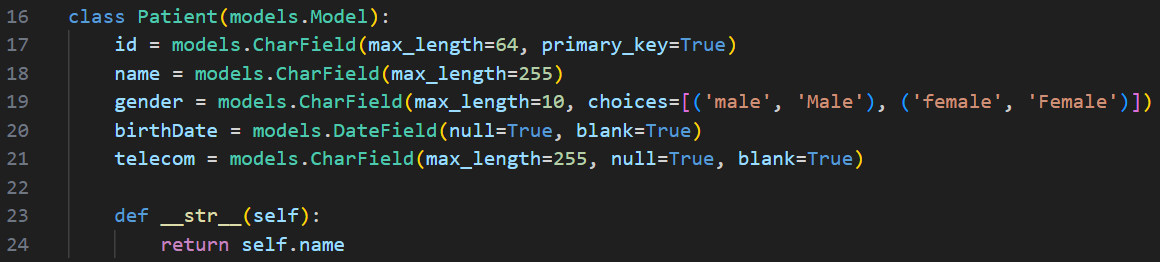
\includegraphics[width=1.0\textwidth]{patient_model.png}
\end{figure}

\subsection{Az időpontfoglalás adatainak tárolása}

Az időpontfoglalás adatait három modellben tárolja az alkalmazás:

\begin{itemize}
	\item Treatment modell: A kezelés típusát tárolja, amire időpontokat lehet foglalni. A kezeléseket az adminisztrátor viszi fel az adatbázisba. A Treatment-nek is van egy $id$ adattagja amibe generálódik automatikusan az uuid4, ezen kívül tárol egy nevet, leírást, egy hosszt, ami azt tárolja, hogy mennyi ideig tart, illetve egy árat ami forintban értendő. Ez a modell is FHIR szabványt követ.
	\item Appointment modell: A lefoglalt időpontot tárolja. Ez az osztálypéldány a páciensek időpontfoglalásának a hatására jön létre. Tárolja a saját id-ját ami automatikusan generálódik a számára amikor létrejön, ezen kvívül van egy $patient$ adattagja ami az időpontot lefoglaló páciens id-ját tárolja. A $practitioner$ adattag ahhoz az orvoshoz kapcsolódik ForeignKey-ként, akihez a páciens időpontot foglalt. Erre azért volt szükség, hogy ha töröljük az orvost az adatbázisból, akkor a hozzá foglalt időpontok is törlődjenek automatikusan. A $treatment$ is hasonló, de a lefoglalt kezeléshez kapcsolódik ForeignKey-ként. A start és end adattagok \texttt{models.DateTimeField} típusúak, és az időpont kezdetét, és végét tárolják. A $status$ karaktersorozat típusú adattag az időpont státuszát tárolja, ami ha "foglalt", akkor nem lehet rá időpontot foglalni. A $custom\_description$ egy TextField típusú adattag, ami a kezeléstörténet tárolására szolgál. Ez az adattag a példány létrehozásakor üres, és a kezelést végző orvos tudja szerkeszteni, a páciensnek csak a megtekintéséhez van joga. Ez a modell is FHIR szabványt követ.
	\item PaymentStatus modell: Ez már nem FHIR szabvány szerinti, viszont szükséges, mert ez tárolja a lefoglalt időpont fizetési státuszát. Tartalmaz egy $appointment$ nevű, \texttt{models.OneToOneField} típusú adattagot, ami által az időponthoz kapcsolódik. (Időpont foglalás esetén automatikusan jön létre az osztálypéldány) Emellett tartalmaz egy bool típusú adattagot aminek $is\_paid$ a neve, és azt tárolja hogy a felhasználó kifizette-e az időpontjára lefoglalt kezelés árát. Ha "true" az értéke, akkor kifizette, ha "false", akkor nem.
\end{itemize}

\subsection{Az orvosok munkaidejének tárolása}

Az orvosok munkaidejének tárolása a WorkingHours modellben történik. Az orvos a "working\_hours.html" oldalon kiválaszthat egy dátumot, és arra a napra beállíthatja a saját munkaidejét. A modell tartalmaz egy $doctor$ nevű, \texttt{models.ForeignKey} típusú adattagot, ami által hozzá kapcsolódik az orvosnak létrejött Doctor osztálypéldányhoz. Van egy $date$ adattagja, amiben azt a dátumot tárolja, amelyikre a munkaidő be lett állítva. Ezek mellett van egy $start$, és egy $end$ adattag, amik értelem szerűen a munkaidő kezdési, és befejezési időpontját tárolják. Ez a modell fontos, mert a páciensek számára megjelenő elérhető időpontok ez alapján jelennek meg.
